\section{Methods}\label{sec:methods}

\subsection{Device model}\label{sec:model}
Each analog weight is one device with a normalised state $u\in[-1,1]$ between its own bounds. Its conductance is
$g=g_{\min}+\tfrac{u+1}{2}(g_{\max}-g_{\min})$, and the weight is read differentially as $w=\alpha\,(g-g_{\mathrm{ref}})$. One
nominal pulse moves $u$ by $k=2/n_{\mathrm{states}}$ at mid-range. With asymmetry $a$ the up and down steps are
$k_\pm=k\,s\,(1\pm a/2)$, where $s$ is a per-device step factor with spread $\sigma_{\mathrm{d2d}}$. With saturation (soft
bounds) the steps depend on the state:
\begin{equation}
\Delta u_+ = k_+\,(1-\gamma_+ u),\qquad \Delta u_- = -k_-\,(1+\gamma_- u).
\end{equation}
The per-device slopes $\gamma_\pm$ have a relative spread $\sigma_\gamma$. A device's symmetry point, where an up and a down
pulse cancel, is $u^*=(k_+-k_-)/(k_+\gamma_++k_-\gamma_-)$. The reference $g_{\mathrm{ref}}$ is set at $g(u^*)$ plus a calibration
error of standard deviation $\sigma_r$, in units of the half-range. A constant-step device has no symmetry point and is
referenced at mid-range.

\begin{itemize}
\item \textbf{Several pulses in one update.} When a device receives $n_+$ up and $n_-$ down pulses in one update, the pulses are
      taken as uniformly interleaved, and $\mathrm{d}u/\mathrm{d}s=A-Bu$ is solved exactly over the batch, with
      $A=k_+n_+-k_-n_-$ and $B=k_+\gamma_+n_++k_-\gamma_-n_-$.
\item \textbf{Write noise.} Cycle-to-cycle noise adds a Gaussian with standard deviation $c_{2c}$ times the local step, growing
      as the square root of the pulse count.
\item \textbf{Drift.} Retention loss relaxes $u$ toward the bare state $u=-1$ with a time constant $\tau$ in training steps.
\item \textbf{Bounds.} The bounds $g_{\min}$, $g_{\max}$ carry a device-to-device spread.
\end{itemize}

\paragraph{The AIHWKIT LinearStepDevice (revision).} The two devices taken from AIHWKIT presets (Li-ECRAM, MO-ECRAM) use
AIHWKIT's own parameterisation instead: the state is the weight itself, with hard bounds $b_{\max}=w_{\max}(1+\sigma_b\xi)$ and
$b_{\min}=w_{\min}(1+\sigma_b\xi)$ around shifted means ($w_{\max}=\RVliWmax$, $w_{\min}=\RVliWmin$ for Li-ECRAM, so that the
symmetry point is at zero), steps $k(1\pm\beta+\sigma_{\mathrm{d2d}}\xi)$, and slopes divided by the mean bounds,
$\Delta w_+=k_+(1-|\gamma_++\sigma_{\gamma+}\xi|\,w/w_{\max})$ and $\Delta w_-=-k_-(1+|\gamma_-+\sigma_{\gamma-}\xi|\,w/|w_{\min}|)$,
with multiplicative write noise.

Forward and backward passes read the weights ideally, in fp32. Read noise and DAC/ADC quantisation are outside the scope of this
study, which isolates the \emph{update}; the energy projection (Section~\ref{sec:energy}) nevertheless prices finite-precision
reads, so accuracy and energy rest on different read assumptions. Biases, layer norms and the language model's position
table are digital.

\subsection{The update}\label{sec:update}
We use the stochastic pulse-coincidence scheme of~\cite{gokmen2016}. Each sample (row) offers $BL=31$ pulse slots. Input $i$
fires with probability $p_{x,i}\propto|x_i|$ and error $j$ with probability $p_{d,j}\propto|d_j|$, with the scaling split equally
between the two streams (update management). Weight $ij$ therefore receives coincidences with mean
$\eta\,|x_i d_j|/(\alpha k)$. Up and down counts are kept separate, so asymmetry is never cancelled digitally. Within a batch the
counts of all samples are summed and drawn from a Poisson distribution with the requested mean. A mini-batch therefore only
groups pulses; it does not average gradients.

This is a surrogate, not a pulse-by-pulse simulation. The mean is exact only while the largest pre-clamp slot probability is at
most one, i.e.\ $(\eta/\alpha k)\max|x|\max|d|\le BL$; beyond that the probabilities are clipped and part of the update is lost.
The repaired simulator records, per layer, the fraction of updates that clipped and the lost fraction of the requested update
(Section~\ref{sec:main}). Discrete pulses do not commute on a state-dependent device (on a 20-level soft-bounds device one up
then one down pulse from $u=0.4$ ends at \RVorderUpDn, the reverse order at \RVorderDnUp, and the batch solution at \RVorderBatch), and independent
per-cell Poisson draws ignore the correlations of shared row and column pulse streams. A larger variance than the binomial one
is therefore not claimed to be conservative. Section~\ref{sec:fidelity} compares the surrogate with explicit pulse streams on
training cases.

\subsection{Algorithms}\label{sec:algos}
\begin{description}
\item[SGD.] The pulses go directly into the weight devices.
\item[TTv1~\cite{gokmen2020}.] The pulses go into an array $A$, and the forward weight is $C+\gamma A$. Every batch, $n_c$ columns
      $j$ of $A$ are read and added to $C$ by a pulsed outer product, $\lambda A_{:,j}\,e_j^{\top}$. $A$ is never reset.
\item[TTv2 (local variant of~\cite{gokmen2021}).] Each read column is added to a digital buffer,
      $H_{:,j}\mathrel{+}=\lambda A_{:,j}/(\alpha k)$. $C$ receives up to 31 pulses where $|H|\ge1$, and $H$ keeps the remainder.
      Optionally the read column of $A$ is reset after the read. Published TTv2 uses single-pulse transfers, forgets a buffer
      element after it fires and does not reset $A$; we name ours a variant and run the published-style form beside it in the
      diagnostic (Appendix~\ref{app:revision}).
\item[The reset of $A$.] The repaired \emph{pulse reset} uses the
      transfer's own read: a sign-directed train of $\mathrm{round}(|A_{ij}|/\alpha k)$ pulses toward the read zero, re-read
      and corrected once, at most 62 pulses per weight, every pulse applied through the device dynamics (with its write noise,
      state-dependent step and device spread) and counted. The original simulator's \emph{ideal reset} (Appendix~\ref{app:revision}) is reported only as a labelled variant.
\item[c-TTv2~\cite{rasch2024}.] Chopper signs $c_j\in\{\pm1\}$ modulate the inputs of the $A$ update ($c\odot x$) and demodulate
      the reads ($c_jA_{:,j}$). Each read column's chopper flips with probability $\rho$.
\item[AGAD~\cite{rasch2024}.] The choppers of c-TTv2, plus a digital leaky average of the reads,
      $p_j\leftarrow(1-\beta)p_j+\beta A_{:,j}$. The read is $z_j=c_j(A_{:,j}-p^{\mathrm{ref}}_j)$, and $p^{\mathrm{ref}}_j$ is
      reset to $p_j$ whenever $c_j$ flips.
\end{description}
In the main experiments every TT-family $A$ array uses a learning rate $1/\lambda$ times larger, so that $\lambda\times$ (the $A$
rate) equals the SGD rate; the TTv1 configuration of the published benchmark (Section~\ref{sec:validation}) is the exception
($\eta=0.01$, $\lambda=0.02$, $A$ rate equal to $\eta$). The settings, including the choice between the pulse reset and no
reset, were chosen once on MNIST validation with a mid-quality device that is not in the catalog (Section~\ref{sec:protocol};
Appendix~\ref{app:selection}). We implemented the algorithms from the papers' text; we did not use the authors' code. Figure~\ref{fig:arch} shows which
parts are simulated as device operations and which are digital.
\begin{figure}[t]\centering
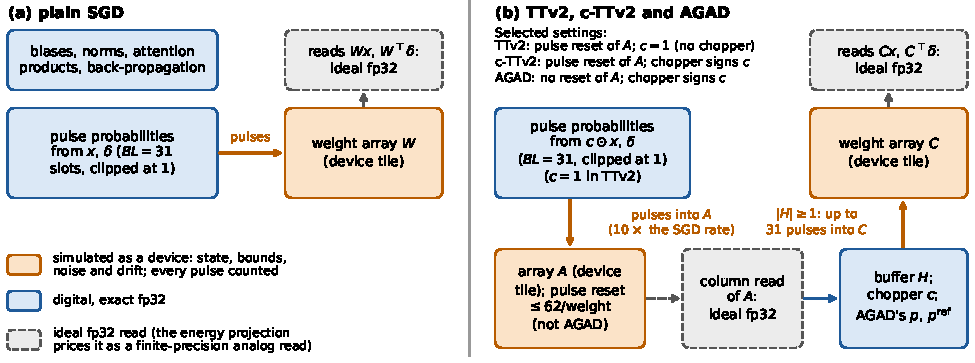
\includegraphics[width=\linewidth]{figs/fig_arch}
\caption{Device operations and digital ones, for one learned weight matrix: (a) plain SGD; (b) TTv2, c-TTv2 and AGAD as run
here, with forward weight $C$ (TTv1, used only in Section~\ref{sec:validation}, has no buffer and no reset). In the selected
configurations (Table~\ref{tab:rev_selection}) TTv2 and c-TTv2 reset $A$ with pulses and AGAD does not reset it; in the
common notation $c\odot x$, $c=\mathbf{1}$ for TTv2, and c-TTv2 and AGAD use chopper signs. Pulse probabilities
are computed digitally; the pulses go through the device model; the forward and backward reads are ideal fp32 products of the
device state; biases, layer norms, nonlinearities, attention products and the LM's position table are digital. The energy
projection (Section~\ref{sec:energy}) prices the reads as finite-precision analog reads, the pulses at device energies and, for
the TT family, one ADC conversion and one buffer update per read weight.}\label{fig:arch}
\end{figure}

\subsection{Device catalog and provenance}\label{sec:catalog}
Table~\ref{tab:rev_catalog} lists the devices as every revised run uses them. Every field carries a provenance label:
\begin{itemize}
\item MEASURED: reported in the paper;
\item FIT: from the AIHWKIT presets fitted to the published devices~\cite{rasch2021aihwkit};
\item CLAIM: a qualitative statement in the paper, translated by us;
\item ESTIMATE: ours;
\item ASSUMED: for example, the 2\% reference error given to every device.
\end{itemize}
The protonic device of~\cite{onen2022} is mostly estimated: the paper reports a thousand up and a thousand down pulses that are
``nearly linear and symmetric'', but no write-noise or variability statistics, and its finite retention is replaced by no
drift. We therefore call it a \emph{protonic-inspired scenario}; a thousand applied pulses are not a demonstration of a
thousand independently programmable states. The original field copy of the Li-ECRAM and MO-ECRAM
rows is kept, labelled as superseded, in Table~\ref{tab:catalog} (Appendix~\ref{app:original}); the revised runs use the one-to-one AIHWKIT mapping above (bounds $[\RVliWmin, \RVliWmax]$ and $[\RVmoWmin, \RVmoWmax]$,
absolute slope spread \RVliGammaDtod). Widrow's memistor is given two specifications,
one as he described it and one pessimistic, together with a pencil-lead cell built today with modern hobby materials
(Appendix~\ref{app:bench}).

% generated by revision2/analyze_rev2.py from records/revision/CATALOG-REV.json (do not edit)
\begin{table*}[t]\centering\footnotesize\caption{Revised device catalog, the configuration of every revised run (simulator units; provenance per field in records/revision/CATALOG-REV.json). $^*$ AIHWKIT's presets mapped one to one onto its LinearStepDevice (shifted bounds, bound-scaled slopes, device spread 0.05 of the slopes and 0.02 of the asymmetry); the others use the paper's model with bounds $[-1,1]$. Columns: levels $n_{\mathrm{st}}$, asymmetry $a$ (device spread), saturation $\gamma_+/\gamma_-$, bounds, write noise $c_{2c}$, step spread $\sigma_{\mathrm{d2d}}$, reference error $\sigma_r$; no drift. The original field-copy catalog is Table~\ref{tab:catalog} (Appendix~\ref{app:original}).}\label{tab:rev_catalog}
\begin{tabular}{llrllllll}\toprule Device & Label & $n_{\mathrm{st}}$ & $a$ & $\gamma_+/\gamma_-$ & bounds & $c_{2c}$ & $\sigma_{\mathrm{d2d}}$ & $\sigma_r$\\\midrule
Li-ECRAM$^*$ & PUBLISHED-FIT & 1000 & 0 & 0.12/0.51 & [-0.83, 1.17] & 0.3 & 0.1 & 0.02\\
MO-ECRAM$^*$ & PUBLISHED-FIT & 7089 & 0 & 0.42/0.73 & [-0.83, 1.17] & 2 & 0.1 & 0.02\\
Protonic-inspired & PARTLY-PUBLISHED & 1000 & 0.05 & 0.20/0.20 & [-1, 1] & 0.3 & 0.1 & 0.02\\
W/WO$_x$ ECRAM & PUBLISHED-FIT & 256 & 0 & 0.63/0.63 & [-1, 1] & 2.048 & 0.023 & 0.02\\
Memistor (optimistic) & CLAIM+ESTIMATE & 1000 & 0.05 & 0.10/0.10 & [-1, 1] & 0.3 & 0.2 & 0.02\\
\bottomrule\end{tabular}\end{table*}


\subsection{Tasks and baselines}\label{sec:tasks}
\begin{description}
\item[MNIST~\cite{lecun1998}.] A 784--256--128--10 tanh MLP; 10 epochs, batch 128, on 55{,}000 training images. 5{,}000 held-out
      training images form the validation set, and the 10{,}000 test images are the test set.
\item[CIFAR-10 subset~\cite{krizhevsky2009}.] Three $3\times3$ convolutions with $c$, $2c$ and $2c$ channels (base $c=32$),
      computed as crossbar matrix products over unfolded patches, then two fully connected layers. 30 epochs, batch 128, on the
      first 10{,}000 images of training batches 1--2. The next 2{,}000 images are the validation set, and the 10{,}000-image
      test set is the test set.
\item[Character LM.] A byte-level, two-layer transformer~\cite{vaswani2017} of width $d$ (base 128) and context 128, trained on
      8\,MB of enwik8~\cite{mahoney2011}, which is human-written Wikipedia text of 2006. 3{,}000 steps of $32\times128$ bytes, each window starting at a uniformly random position. The start's upper bound is
      one short, so the last window of the training slice is never drawn and the slice's final byte is
      never a target; no held-out byte is affected.
      Every learned weight matrix uses the device model, including the embedding and the head; the activation-dependent
      attention products and the other operations are digital. Validation is the slice's last 0.5\,MB, held out from
      training in selection runs. Test is a separate 0.5\,MB slice.
\end{description}
The first baseline (``FP-SGD'') is the same network, initialisation, data order and update rule with an exact floating-point
weight update. The second is Adam~\cite{kingma2014} on digital twins with the same initialisation and data order and its own
learning rate selected on validation; in the revision it is reported for all three tasks, beside FP-SGD. The gap is FP accuracy minus device
accuracy for classification, in percentage points. For the LM it is the device's bits per byte relative to FP's, minus one, in
percent.

\subsection{Protocol and statistics}\label{sec:protocol}
Every experiment was pre-registered in a committed plan before it ran (Section~\ref{sec:availability}).
\begin{itemize}
\item \textbf{Hyperparameters} were chosen on validation splits only, with an edge rule: whenever the best value of a grid lies
      at its edge, the next half-decade point is added. The learning rate of every device arm in the main table is the FP
      validation choice. The scale study instead tunes each arm separately.
\item \textbf{Statistics.} The main table uses five seeds per arm. Gaps are paired by seed, and we report the mean and a 95\% Student-$t$ interval (the $t$ quantile computed exactly). A cell PASSES when the whole interval lies below the gap line (2\,pp for classification, 5\% for
      the LM), FAILS when it lies wholly above, and is UNRESOLVED otherwise.
\item \textbf{Multiplicity.} We make no correction for multiplicity. The intervals describe each cell, not the family, and a
      best cell chosen among many is optimistic.
\item \textbf{Random streams (revision).} Each seed defines separate generators for the logical initialisation, the data
      order, each tile's device population and the pulse and noise draws, so the paired gap compares runs that share their
      initial weights and their data.
\item \textbf{Width (revision).} The endpoint contrast $D$ (gap at the widest minus the narrowest width) is tested for
      equivalence (TOST at 5\,\%, margins equal to the gap lines); ``no evidence of growth beyond the margin'' when only the upper
      bound is under the margin; never ``flat''.
\item \textbf{Sensitivity (revision).} Each grid point is labelled against the \emph{absolute} line with 3 seeds paired with
      FP-SGD of the same seed; a threshold is the weakest value that passes with every value toward the best end passing.
\end{itemize}

\subsection{Simulator checks}\label{sec:checks}
The simulator is checked by \nChecks{} checks, and each check is shown to fail on at least one deliberately planted fault
(\nFaults{} faults in all). Examples of what the checks cover:
\begin{itemize}
\item the exact-update arm equals PyTorch SGD;
\item the mean pulse update equals the SGD step;
\item alternating pulses converge to the analytic symmetry point, including with per-device slopes;
\item write noise grows as $\sqrt n$;
\item drift relaxes to the bare state;
\item a static read offset is integrated by TTv2, mostly cancelled by c-TTv2 and nearly fully cancelled by AGAD;
\item TTv1 moves $C$ along $+\lambda A$;
\item the SGD and TTv2 paths are bit-identical to the earlier code that produced our preliminary results.
\end{itemize}
The planted faults include a swapped pulse sign, a dropped chopper demodulation and a never-updated AGAD reference.
Both suites run at the start of every compute session and stop it on any failure (Appendix~\ref{app:checks}). The revision
adds \RVnChecks{} checks of the repairs (matched initialisation and data order across arms, a shared device population across
algorithms, resets that charge exactly the pulses they apply, the AIHWKIT LinearStepDevice recurrence, the clipping statistics,
the published-style buffer, the re-centred symmetry point, and a bit-exact replay of the original simulator), each shown to
fail on the old behaviour or a planted fault (Appendix~\ref{app:revision}). These checks test the implementation; they do not
validate the physical model.
